%This sections concerns the design of our MiniTwit system. Wherein we describe and discuss the design and architecture of the system. Following that a reflection of the different tools and dependencies used for the project. Finally we assess the current state of the system, using INSERT PERFORMANCE METRIC.
%MSc students should argue for the choice of technologies and decisions for at least all cases for which we asked you to do so in the tasks at the end of each session.

\subsection{Design \& Architecture}
%Our Minitwit system evolved during the course into the current architecture shown in Fig. \ref{fig:Deployment}. It features a web interface that communicates with a backend API; the API reads and writes to a database. To enhance availability and reduce downtime, the system is deployed using a hot–cold server configuration, facilitated through \textbf{keepalived}. This setup ensures that a backup instance can be quickly activated if the primary server (Droplet) fails. The entire system is hosted on DigitalOcean, where we also utilize a PostgreSQL database to manage persistent data storage. In addition to its core functionality, the system includes support for both monitoring and logging, which are discussed in more detail in Sections \ref{sec:monitoring} and \ref{sec:logging}. 

Our Minitwit system evolved during the course into the current architecture shown in Fig. \ref{fig:Deployment}. The entire system is hosted on DigitalOcean, where a web interface communicates with a backend API; the API reads and writes to a PostgreSQL database where persistent data is managed. In addition both monitoring and logging are integrated, including volumes to store logs and metrics. Fig. \ref{fig:Deployment} shows how the servers (Droplets) are set up; each runs eight containers when active as well as a Keepalived daemon for the failover mechanism. At all times one server is active, serving the Minitwit web application and accessing the database. To ensure availability floating IPs are used to point to the appropriate server during failures and updates. All features mentioned here are expanded upon in coming sections.

\begin{figure}[!htb]
    \centering
    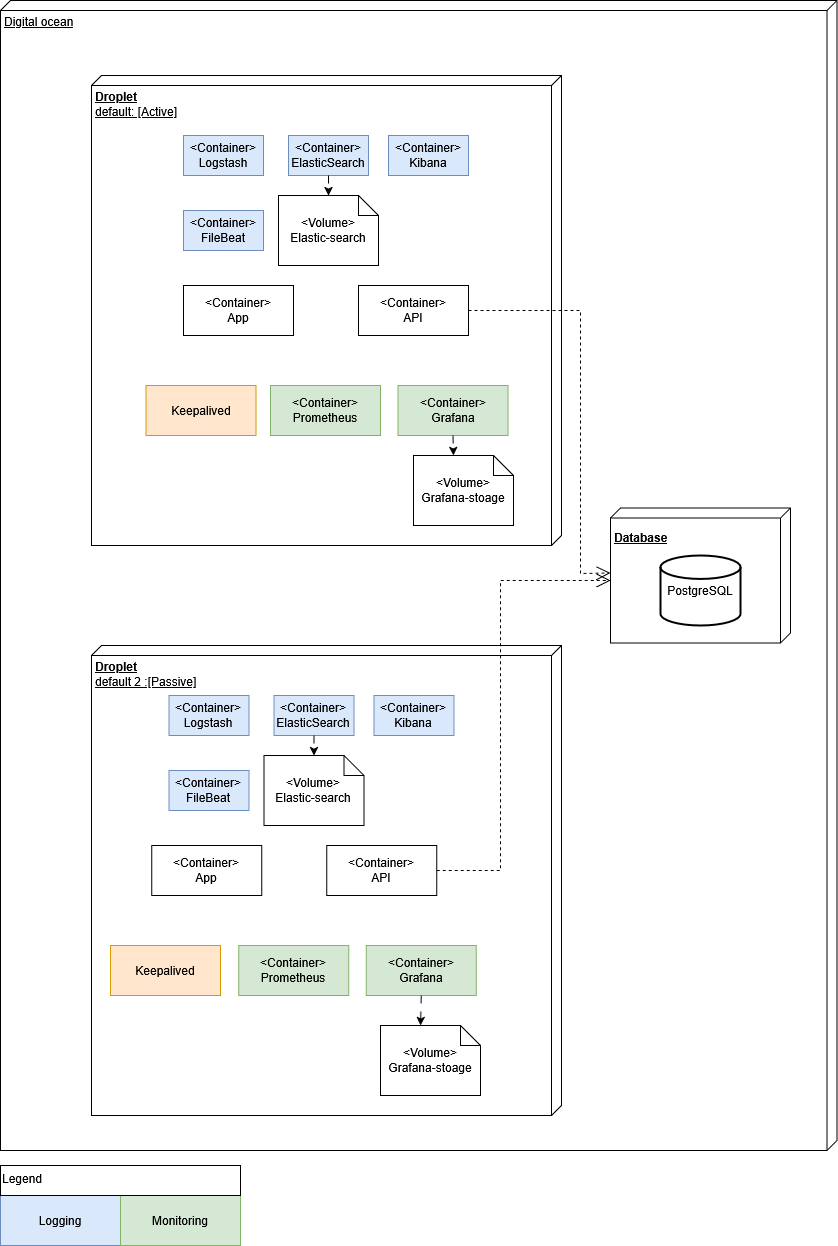
\includegraphics[width=0.5\linewidth]{Images/Deployment.png}
    \caption{Deployment diagram}
    \label{fig:Deployment}
\end{figure}

%gwen&tore
%static view
%- overall abstract system diagram DONE
%- UML deployment diagram (incl load-balancing)

\subsection{Dependencies \& Tools}
%iulia&olivia
%All dependencies of your ITU-MiniTwit systems on all levels of abstraction and development stages. That is, list and briefly describe all technologies and tools you applied and depend on.`

\subsubsection*{Development \& Runtime}
\begin{itemize}
  \item \textbf{Go (Golang)} – Primary language for the application.
  \item \textbf{GORM} – ORM for Go used to interact with the database.
  \item \textbf{Gorilla Mux} – HTTP router and URL matcher for Go, used to handle routing in the backend API.
  \item \textbf{Python} – Used for testing, especially API and UI validation.
  \item \textbf{Docker \& Docker Compose} – Containerization of all services and orchestration for local and CI environments.
\end{itemize}

\subsubsection*{Infrastructure}
\begin{itemize}
  \item \textbf{Terraform} – Infrastructure as Code to provision and manage DigitalOcean droplets, floating IPs, and DigitalOcean Spaces.
  \item \textbf{DigitalOcean} – Cloud provider hosting the production infrastructure, including our high availability setup.
  \item \textbf{Vagrant} – Used initially to provision reproducible local development environments.
  \item \textbf{Keepalived} – Provides failover between active and standby droplets using floating IP reassignment.
  \item \textbf{Docker Hub} - Used to store the Docker images.
\end{itemize}

\subsubsection*{CI/CD \& Automation}
\begin{itemize}
  \item \textbf{GitHub Actions} – Automates testing, building, deploying, and releasing workflows.
  \item \textbf{gofmt} – Enforces Go code formatting standards.
  \item \textbf{golangci-lint} – Static analysis aggregator for Go code quality.
  \item \textbf{dockerfilelint} – Linter for validating Dockerfiles.
  \item \textbf{GitHub CLI} – Used for automated GitHub release creation. 
  \item \textbf{SonarQube} – Used to automatically analyze code quality.
\end{itemize}

\subsubsection*{Testing \& Validation}
\begin{itemize}
  \item \textbf{Go test} – For backend unit and integration tests.
  \item \textbf{pytest} – Runs API-level tests written in Python.
  \item \textbf{Selenium (with Firefox + Geckodriver)} – Powers UI and end-to-end testing in a headless browser.
  \item \textbf{unittest (Python)} – Traditional functional tests.
  \item \textbf{SQLite3} – Lightweight database used in testing environments to verify correctness.
\end{itemize}

\subsubsection*{Monitoring \& Logging}
\begin{itemize}
  \item \textbf{Prometheus} – Collects metrics from application containers, especially health and performance indicators.
  \item \textbf{Grafana} – Provides dashboards and visualizations of Prometheus metrics at \texttt{localhost:3000}.
  \item \textbf{Elasticsearch} – Central log storage and indexing engine for collecting application logs.
  \item \textbf{Logstash} – Processes and forwards logs from containers into Elasticsearch.
  \item \textbf{Filebeat} – Lightweight log shipper running on containers to collect logs.
  \item \textbf{Kibana} – UI for querying and visualizing logs from Elasticsearch (at \texttt{localhost:5601}).
  \item \textbf{Keepalived} – Also monitors app health to trigger failover, contributing indirectly to availability observability.
\end{itemize}

\subsection{Subsystems Interactions}
%gwen&tore
%dynamic view
We chose two common scenarios to illustrate a dynamic view of our system. First the sequence diagram below, Fig. \ref{fig:seq_user}, shows the flow of events triggered by a user when they attempt to send a new message. It starts with the User pressing submit, having filled out the HTML form which makes the app issue a POST request to the API. Upon receiving the request an initial logging event records the attempt. The API queries the PostgreSQL database to retrieve the User's ID which it then uses to create a new message entry. Once the message is successfully saved in the database, confirmation that the message was stored without error is logged and two separate counters used for system monitoring are updated. Finally, the API returns a 204 No Content HTTP status code to the Simulator to signal that the message was properly processed.

\begin{figure}[!htb]
    \centering
    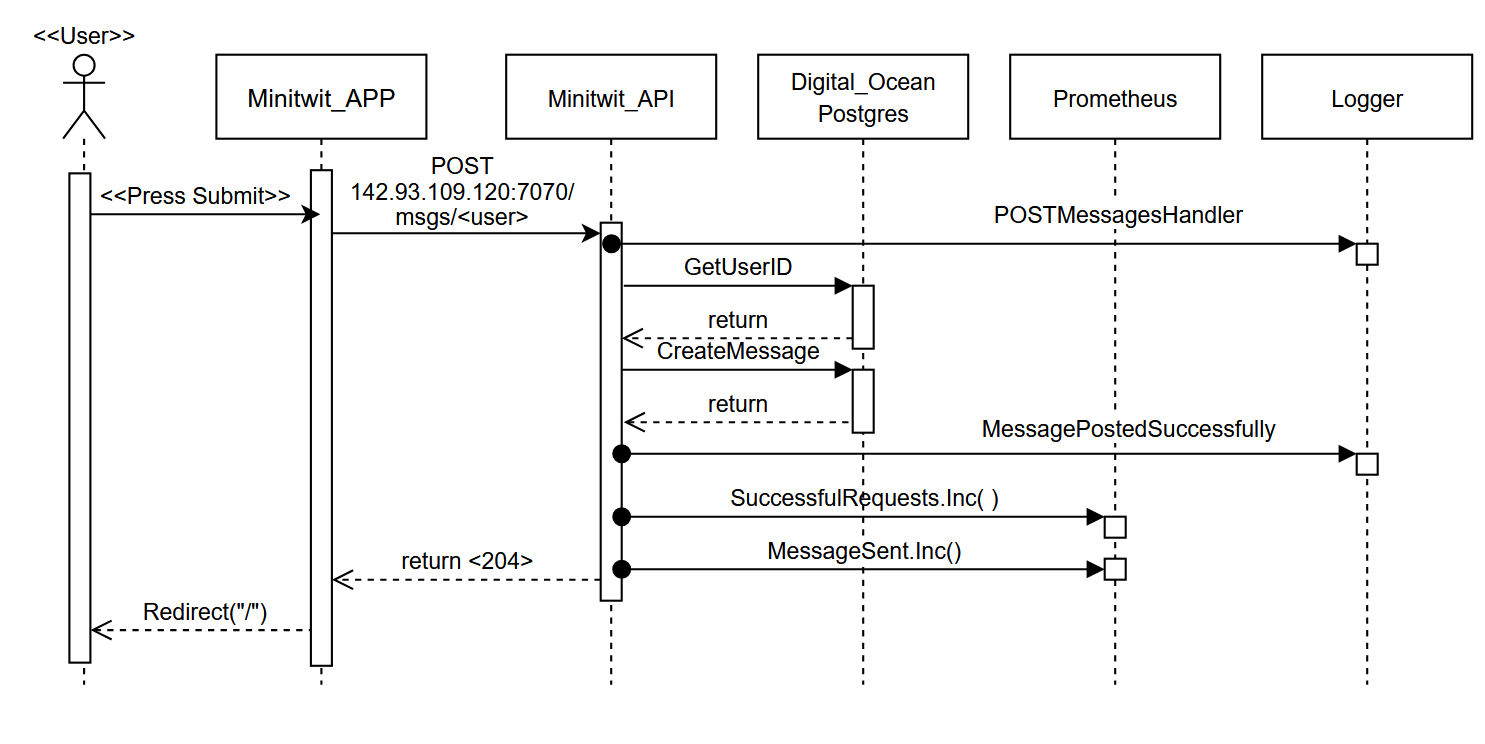
\includegraphics[width=0.9\linewidth]{Images/seq_user.png}
    \caption{Sequence diagram of a successful sent message from the user's perspective}
    \label{fig:seq_user}
\end{figure}

The next sequence diagram, Fig. \ref{fig:seq_fail}, shows a common interaction between the Simulator and our system this semester. When an error prevents a User from being created, the Simulator may later attempt to send a message through a \textbf{POST} request at the "\textit{/msgs/<<User>>}" endpoint. This is unsuccessful since the User does not exist and therefore cannot post.\\ \\ 

\begin{figure} [!htb]
    \centering
    \includegraphics[width=0.9\linewidth]{Images/Seq_fail.png}
    \caption{Sequence diagram of the simulator trying to post a message as a non-existent user.}
    \label{fig:seq_fail}
\end{figure}
\newpage
\subsection{Current State}
%MAX
%Describe the current state of your systems, for example using results of static analysis and quality assessments.
We’ve been using SonarCloud since March 28 to monitor code quality. The Quality Gate passes, but deeper analysis highlights several areas for improvement:

\begin{itemize}
    \item \textbf{Code Duplication:} Currently at 4.4\%, exceeding the 3\% recommended threshold. New code remains within limits, but duplication is mainly due to repeated literals and logic across components.
    
    \item \textbf{Maintainability:} 55 open code smells, many flagged as high severity. These are mostly related to repeated strings that should be refactored into constants.
    
    \item \textbf{Reliability:} 10 minor issues, no blockers.
    
    \item \textbf{Security:} No active vulnerabilities, but 21 security hotspots, mostly due to hardcoded credentials in test files (e.g., \texttt{pwd = "super\_safe"}). These don’t impact production but should be reviewed.
\end{itemize}

Summarising the above, the overall maintainability and reliability ratings sit at A, while the security rating is E. Technical debt is estimated at 6.5 hours. The codebase is in stable condition, but is in need of some maintenance to improve long-term quality.



